\documentclass[a4paper,11pt]{article}

% Identificação
\newcommand{\pbtitulo}{Neo4j com Java e Python}
\newcommand{\pbversao}{1.0}

\usepackage{../sty/tutorial}

%----------------------------------------------------------------------
% Início do Documento
%----------------------------------------------------------------------
\begin{document}
	
\maketitle % mostrar o título
\thispagestyle{fancy} % habilitar o cabeçalho/rodapé das páginas

%----------------------------------------------------------------------
% RESUMO DO ARTIGO
%----------------------------------------------------------------------
	
\begin{abstract}
	\initial{N}\textbf{eo4j é um banco do tipo NoSQL que é considerado como um sistema gerenciador para banco de dados Grafo. Oferece aos desenvolvedores e cientistas de dados as ferramentas mais confiáveis e avançadas para criar rapidamente os aplicativos inteligentes e fluxos para aprendizado de máquina. Disponível como um serviço de nuvem totalmente gerenciado ou auto-hospedado. Neste tutorial veremos o que vem a ser o banco NoSQL Neo4j \cite{neo4joficial} e como proceder sua utilização utilizando como pano de fundo a linguagem de programação Java \cite{javaoficial} e Python \cite{pythonoficial}.}
\end{abstract}

%-----------------------------------------------------------------------------
% CONTEÚDO DO ARTIGO
%-----------------------------------------------------------------------------

\section{Parte inicial}
Neo4j foi criador em 2000, quando \textit{Emil Eifrem}, \textit{Johan Svensson} e \textit{Peter Naubauer} começaram a notar uma quantidade significativa de sobrecarga tanto no desempenho quanto ao trabalho exigido em uma de suas aplicações. O primeiro e mais significativo aspecto da sobrecarga pode ser atribuído à incompatibilidade do modelo na forma como o SGBD Relacional estava trabalhando. Observaram que as conexões entre os dados impunham um longo tempo de processamento para as consultas. Além disso, o desempenho dessas ficou pior à medida que as conexões entre os dados se tornaram mais complexas. Finalmente, o tempo e esforço necessários para gerenciar esses relacionamentos colocaram ainda mais sobrecarga no ciclo de vida no desenvolvimento do aplicativo.
\begin{figure}[H]
	\centering
	
\includegraphics[width=0.35\textwidth]{imagens/neo4jlogo}
	\caption{Logo do Neo4j}
\end{figure}

Depois de buscarem alternativas e algumas pesquisas, começaram a construir um projeto denominado \textbf{Neo}. O objetivo era apresentar um banco de dados que oferecesse uma maneira melhor de modelar, armazenar e recuperar dados, ao mesmo tempo em que mantinha todos os conceitos básicos, tais como ACID ou transações, que tornavam os SGBD Relacionais seguros e conhecidos.

Uma transação num banco relacional é essencialmente um grupo de consultas que devem ser bem-sucedidas para serem aplicadas. Se algo em uma transação falhar, toda ela deve também falhar. As transações possuem dois propósitos básicos, ambos envolvendo consistência, apenas de maneiras diferentes: O primeiro é garantir que todas os comandos dentro dessa sejam realmente executados. O segundo diz respeito a duas ações que acontecem ao mesmo tempo: se um banco de dados está sendo consultado simultaneamente por várias fontes, então existe a possibilidade da integridade dos dados ser comprometida.

Os princípios usados no ACID (Atomicidade, Consistência, Isolação e Durabilidade) são relativos ao Teorema CAP, também conhecido como \textit{Teorema de Brewer}. \textit{Eric Brewer} afirmou que é impossível para um sistema de computador distribuído (ou banco de dados) garantir simultaneamente as três condições a seguir:
\begin{itemize}[nolistsep]
	\item \textbf{Disponibilidade} cada solicitação recebe uma resposta sobre se foi bem-sucedida ou falha.
	\item \textbf{Consistência} os dados estão disponíveis para todos os nós ao mesmo tempo.
	\item \textbf{Tolerância de partição} o sistema ainda pode operar apesar de perder contato com outros
nós devido a problemas de rede.
\end{itemize}

Assim pegaram esses conceitos e adicionaram os princípios da \textbf{teoria dos grafos} aplicando-os ao projeto \textbf{Neo}. Graças a este trabalho árduo, os relacionamentos entre dados é a característica levada muito a sério. Em um sentido matemático, a teoria dos grafos é o estudo das estruturas usadas para modelar o  relacionamento entre os objetos. 

Neo4j armazena dados como vértices e arestas ou, na terminologia dos grafos, nós e relacionamentos. Por exemplo donos são representados como nós e carros serão representadas como relacionamentos entre nós de usuários. Assim rapidamente podemos associar todas as pessoas que compraram determinado veículo (com apenas um único relacionamento).

\subsection{O que é um Grafo?}
O primeiro artigo conhecido sobre a teoria dos grafos foi escrito em 1736, chamado de "\textit{As 7 Pontes de Königsberg}" por Leonhard Euler, um matemático e físico, considerado preeminente do século XVIII. A cidade de \textit{Königsberg}, na Prússia (atual Rússia), foi construída no topo do rio \textit{Pregel} e incluía duas grandes ilhas que eram conectadas entre si e ao continente por sete pontes. O problema era conhecer a possibilidade em se cruzar cada uma das sete pontes de Königsberg apenas uma vez e visitar todas as partes da cidade.
\begin{figure}[H]
	\centering
	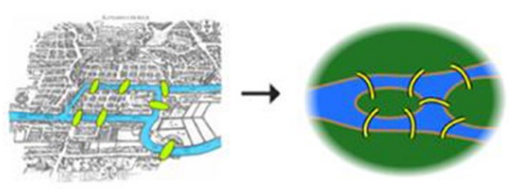
\includegraphics[width=0.5\textwidth]{imagens/pontes}
	\caption{As 7 Pontes de Königsberg}
\end{figure}

Após abstrair o problema em um gráfico, Euler percebeu um padrão, baseado no número de vértices e arestas. No gráfico de Königsberg, existem 4 vértices e 7 arestas. No sentido literal, Euler percebeu que se caminhasse para uma das ilhas e sair para outra, usaria uma ponte de entrada e uma ponte de saída. Essencialmente, para atravessar um caminho sem cruzar uma aresta mais de uma vez, seria então necessário um número par de arestas.

Euler teorizou que percorrer um gráfico inteiramente, usando cada aresta apenas uma vez, depende dos graus de um nó. No contexto de um nó ou vértice, graus se refere à quantidade de arestas que tocam o nó. Se percorrermos um gráfico completamente (usando apenas uma aresta por vez), podemos ter de 0 ou 2 nós com graus ímpares (cruzar um gráfico dessa forma é conhecido como \textit{Caminho de Euler}). 

Nesse contexto, um grafo é composto de nós (ou vértices) e potencialmente arestas que os conectam. Para visualizarmos isso, podemos usar uma seta para indicar que um nó está conectado a outro nó. Por exemplo, se tivéssemos dois nós, A e B, aos quais A está conectado a B com uma aresta, isso poderia ser expresso como A $\triangleright$ B. A direção é mostrada aqui em que A está conectado a B, mas B não está conectado a A. Se as arestas que compõem um gráfico não têm uma direção associada (por exemplo, A $\triangleright$ B é o mesmo que B $\triangleright$ A), então o gráfico é classificado como não direcionado. Se, no entanto, a orientação da aresta tiver algum significado, o gráfico é direcionado.
\begin{figure}[H]
	\centering
	
\includegraphics[width=0.6\textwidth]{imagens/Elementary.jpg}
	\caption{Cena da Série Elementary (CBS)}
\end{figure}

Existem outras aplicações para a teoria dos grafos fora do mundo da matemática. Uma vez que a teoria dos gráficos, em seu nível mais baixo, descreve como os dados se relacionam uns com os outros, pode ser aplicada a uma série de diferentes setores e cenários onde relacionar os dados é importante. Pode ser usada para mapear estruturas químicas, criar diagramas de estradas e até mesmo analisar dados de redes sociais. As aplicações são bastante amplas. 

No Neo4j todos esses conceitos estão amplamente aplicados: \vspace{-1em}
\begin{itemize}
	\item \textbf{Nó} representamos entidades com Nó. Identificamos ao criar nosso modelo de dados. Junto com os relacionamentos, nó é uma das unidades fundamentais que formam um gráfico.
	\item \textbf{Propriedades} representam os atributos do nó e relacionamentos. São pares nome-valor usados para adicionar qualidades a nós ou relacionamentos.
	\item \textbf{Rótulo (label) do nó} Podemos atribuir funções ou tipos a um nó usando um ou mais rótulos. São utilizados para agrupar nós onde todos com o mesmo rótulo pertencem ao mesmo grupo.
	\item \textbf{Relação} Usamos um relacionamento para conectar dois nós. Deve ter exatamente um tipo de relacionamento.
\end{itemize}
	
\subsection{Criar o contêiner Docker}
A forma mais simples para obtermos o Neo4J é através de um contêiner no Docker, deste modo podemos ter várias versões do banco instalada e controlar mais facilmente qual banco está ativo ou não. E ainda colhemos o benefício adicional de não termos absolutamente nada deixando sujeira em nosso sistema operacional ou áreas de memória.

Baixar a imagem oficial: \\
\codigo{\$ docker pull neo4j}

Antes de criarmos o contêiner precisamos criar uma pasta em nosso disco para hospedar o banco, por exemplo minha pasta chama-se: "/home/fernando/neo4j". Deste modo a criação do contêiner será: \\
\codigo{\$ docker run -d -p 7687:7687 -p 7474:7474 -v \$HOME/neo4j/data:/data \\ -v \$HOME/neo4j/logs:/logs -v \$HOME/neo4j/import:/import \\ -v \$HOME/neo4j/plugins:/plugins --env NEO4J\_AUTH=neo4j/test --name meu-neo4j neo4j}

Podemos entrar no \textit{Cypher-shell} dentro do nosso contêiner: \\
\codigo{\$ docker exec -it meu-neo4j bash}

Acessar o Cypher-shell: \\
\codigo{\$ cypher-shell -u neo4j -p test}

Quando criamos o contêiner usamos a opção: \codigo{--env NEO4J\_AUTH=neo4j/test}, neste ponto indicamos a senha \textbf{test} para o \textit{Cypher-shell} e devemos usá-la quando entramos neste. Executamos uma consulta para verificarmos que está tudo OK: \\
\codigo{neo4j> MATCH (n) RETURN count(n);}

E obtemos:
\begin{figure}[H]
	\centering
	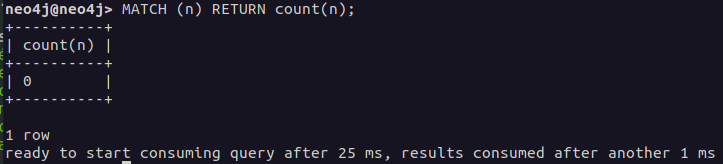
\includegraphics[width=0.7\textwidth]{imagens/cyphershell}
	\caption{Execução do comando no Cypher-shell}
\end{figure}

Podemos sair do \textit{Cypher-shell} com o comando: \\
\codigo{neo4j> :exit}

E com o comando: \\
\codigo{\$ exit}

Para sairmos do contêiner. Na seção \textbf{Cypher} investigaremos mais sobre essa linguagem. Podemos parar o contêiner com: \\
\codigo{\$ docker stop meu-neo4j} 

Ou iniciá-lo novamente: \\
\codigo{\$ docker start meu-neo4j}

\subsection{Gerenciar o Neo4j}
Uma vez que subimos nosso contêiner, após alguns segundos, está a nossa disposição uma das ferramentas mais úteis incluídas em um banco de dados o "Neo4j Browser", no endereço: \url{http://localhost:7474}.
\begin{figure}[H]
	\centering
	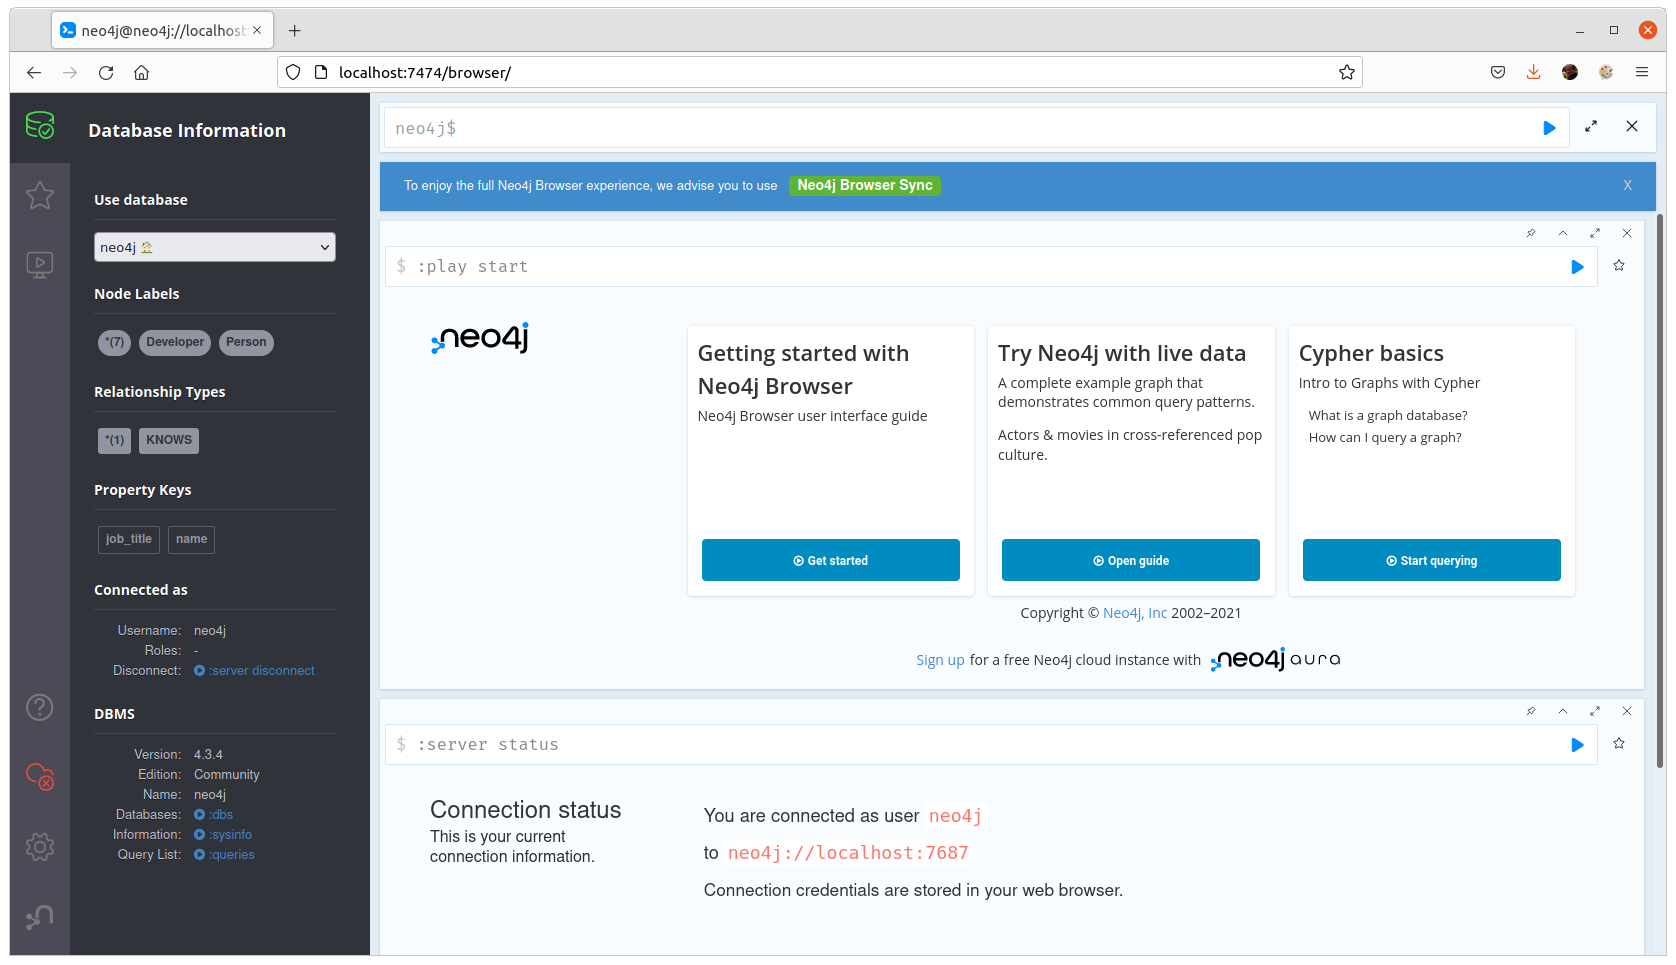
\includegraphics[width=0.7\textwidth]{imagens/browser}
	\caption{Neo4j Browser}
\end{figure}

É possível com este aplicativo realizar melhorias significativas para os recursos, velocidade e testes no banco através dessa ferramenta de visualização com base na Web. Na barra superior da janela principal, devemos dar o máximo de atenção na indicação \textbf{neo4j$\textdollar$ }pois neste ponto podemos inserir comandos em linguagem \textbf{Cypher}.

\section{Cypher}
A linguagem utilizada para trabalhar com o Neo4j chama-se Cypher, a primeira representação que devemos conhecer é:
\begin{itemize}[nolistsep]
	\item \textbf{Parênteses} devem ser usados para os nós.
	\item \textbf{Chaves} devem ser usadas para as propriedades.
	\item \textbf{Colchetes} devem ser usados para os relacionamentos.
\end{itemize}

Uma dica simples podemos tentar comparar com os comandos SQL, porém essa linguagem nada tem a ver, por exemplo, um comando básico usado frequentemente é:
\begin{lstlisting}[]
MATCH (a)-[:DONA]->(b) RETURN a, b;
\end{lstlisting}

Realiza uma consulta que mostra como obter todos os nós que estão relacionados entre si por um determinado relacionamento chamado \textbf{DONA}. Mas vamos começar com muita calma e ir avançado, para executar qualquer comando, na barra de comandos do \textit{Neoj Browser} digitamos:
\begin{lstlisting}[]
MATCH (n) RETURN n;
\end{lstlisting}

E pressionamos o botão para executar, o resultado deve ser algo assim:
\begin{figure}[H]
	\centering
	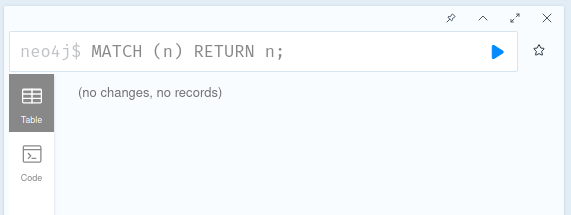
\includegraphics[width=0.4\textwidth]{imagens/consulta}
	\caption{Execução do comando no Neo4j Browser}
\end{figure}

Essa consulta nos mostra que não existe nenhum banco ou registro cadastrado. Em seguida, veremos uma estrutura completa do banco de dados, para facilitar o entendimento tentaremos associar isso aos comandos SQL.

\subsection{Comando CREATE / CREATE UNIQUE}
Este comando é utilizado para criarmos qualquer elemento no banco de dados: nós, relacionamentos, propriedades ou combinações entre eles. Podemos associá-lo com \textbf{INSERT}, porém age de forma bem diferente do SQL, primeiro um Nó (que seria o correspondente a uma entidade) pode ter vários nomes, por exemplo:
\begin{lstlisting}[]
CREATE (:Pessoa:Proprietario);
\end{lstlisting}

Podemos criar algumas propriedades para este nó:
\begin{lstlisting}[]
CREATE (:Pessoa { nome : 'Fernando', modelo_carteira : "AB" });
CREATE (:Pessoa { nome : 'Anselmo', modelo_carteira : "B" });
CREATE (:Automovel { nome : 'Ecosport' });
\end{lstlisting}

Os relacionamentos são criados assim, para a pessoa com o nome "Fernando":
\begin{lstlisting}[]
MATCH (p:Pessoa { nome: "Fernando" }) OPTIONAL MATCH (a:Automovel { nome: "Ecosport" }) CREATE (p)-[:DONA]->(a)
\end{lstlisting}

E para a pessoa com o nome "Anselmo":
\begin{lstlisting}[]
MATCH (p:Pessoa { nome: "Anselmo" }) OPTIONAL MATCH (a:Automovel { nome: "Ecosport" }) CREATE (p)-[:DONA]->(a)
\end{lstlisting}

E com o comando:
\begin{lstlisting}[]
MATCH (n) RETURN n;
\end{lstlisting}

Podemos visualizar o seguinte Grafo:
\begin{figure}[H]
	\centering
	\includegraphics[width=0.3\textwidth]{imagens/relacionamento}
	\caption{Grafo entre Pessoa e Automóvel}
\end{figure}

Também podemos criar simultaneamente todas as pessoas e seus relacionamentos com um único comando que seria:
\begin{lstlisting}[]
CREATE (:Pessoa {nome: "Fernando", modelo_carteira : "AB"})-[:DONA]->(:Automovel {nome: "Ecosport"})<-[:DONA]-(:Pessoa {nome: "Anselmo", modelo_carteira : "B"});
\end{lstlisting}

\subsection{Comando MATCH - Subcomando SET}
Normalmente o comando \textbf{MATCH} é associado com o \textbf{SELECT}, porém faz muito mais já o vimos associado ao \textbf{CREATE}, com sua associação a SET podemos adicionar ou criar propriedades nos nós:
\begin{lstlisting}[]
MATCH (n) WHERE n.nome = "Fernando" SET n.profissao = "Desenvolvedor"
\end{lstlisting}

Se reparar na sintaxe podemos fazer uma associação ao comando \textbf{UPDATE}.

\subsection{Comando MATCH - Para consultas}
Nota-se que este é o principal comando em Cypher, o comando MATCH é extremamente versátil, para retornarmos todas as pessoas com um nome específico:
\begin{lstlisting}[]
MATCH (n:Pessoa {nome: "Fernando"}) RETURN n;
\end{lstlisting}

Retornar um conjunto específico de propriedades (não todas):
\begin{lstlisting}[]
MATCH (p:Pessoa {nome: "Fernando"})
RETURN p.modelo_carteira, p.profissao
\end{lstlisting}

Retornar todas as pessoas que não possuem o valor de alguma propriedade específica:
\begin{lstlisting}[]
MATCH (p:Pessoa) 
WHERE NOT p.nome = 'Anselmo'
RETURN j
\end{lstlisting}

A subcláusula WHERE funciona quase da mesma forma que o SQL, por exemplo, vamos supor que as pessoas tivessem uma propriedade "experiencia" (em anos) e desejamos conhecer todas em um determinado intervalo:
\begin{lstlisting}[]
MATCH (p:Pessoa)
WHERE 3 <= p.experiencia <= 7
RETURN p
\end{lstlisting}

Ou para avaliar a existência de um determinado valor em um relacionamo:
\begin{lstlisting}[]
MATCH (p:Pessoa)-[rel:DONA]->(a:Automovel)
WHERE p.modelo_carteira IS NOT NULL
RETURN p, rel, a;
\end{lstlisting}

Para combinarmos os nós que estão relacionados, independentemente da direção (observe a falta de uma seta) e retornar de ambos os lados:
\begin{lstlisting}[]
MATCH (a)--(b) RETURN a, b;
\end{lstlisting}

Podemos atribuir os relacionamentos a uma variável "r", e isso significa que podem ser retornados da consulta, portanto, se precisamos do relacionamento (ou qualquer uma de suas propriedades):
\begin{lstlisting}[]
MATCH (a)-[r]-(b) RETURN a, r, b;
\end{lstlisting}

Quando não desejamos caracterizar tudo, ou seja somente um certo tipo de relacionamento, adicionamos o padrão ":TIPO". Nesse caso, o tipo é DONA e, como o relacionamento não é necessário posteriormente, o alias é descartado:
\begin{lstlisting}[]
MATCH (a)-[:DONA]->(b) RETURN a, b;
\end{lstlisting}

Em vez de apenas retornar todos os nós envolvidos em um caminho, podemos obter o próprio caminho. Com base no exemplo anterior, isso será transformado em um caminho nomeado:
\begin{lstlisting}[]
MATCH p=(a)-[:DONA]->(b) RETURN p;	
\end{lstlisting}

É possível usar várias cláusulas MATCH em uma consulta, portanto, para retornar dois nós específicos, podemos usar várias causas de correspondência e, em seguida, retornar o resultado: 
\begin{lstlisting}[]
MATCH (a:Pessoa {nome: 'Fernando'})
MATCH (b:Pessoa {nome: 'Anselmo'})
RETURN a, b;
\end{lstlisting}

Que podemos simplificar para:
\begin{lstlisting}[]
MATCH (a:Pessoa {nome: 'Fernando'}),(b:Pessoa {nome: 'Anselmo'}) RETURN a, b;
\end{lstlisting}

Esse comando é extremamente importante pois mostra bem o princípio que discutimos sobre transações, retorna os nós solicitados exatamente como esperamos. Se o segundo MATCH falhar, então o primeiro também falha, e a consulta retorna 0 resultados, pois está procurando por um \textbf{AND} também b, portanto, caso não conseguir encontrar nada em "b" então a consulta não é válida. 

Podemos contornar isso, com a utilização de uma correspondência opcional. Retorna somente se a correspondência estiver presente. Do contrário, retornará \textbf{null}: 
\begin{lstlisting}[]
MATCH (a:Pessoa {nome: 'Fernando'})
OPTIONAL MATCH (b:Pessoa {nome: 'Anselmo'})
RETURN a, b;
\end{lstlisting}

Este sinalizador \textbf{OPTIONAL MATCH} é utilizado para retornar relacionamentos potenciais para um nó. Se apenas o nó pode ter um relacionamento, pode ser usado para remediar isso, assim: 
\begin{lstlisting}[]
MATCH (a:Pessoa {nome: 'Fernando'})
OPTIONAL MATCH (a)-->(x)
RETURN a, x;	
\end{lstlisting}

Assim para todos os nós rotulados como "Pessoa" com o nome de "Fernando", ambos os nós que possuem ou não relacionamentos serão retornados.

\subsection{Comando MATCH - Subcomando DELETE}
Vamos começar limpando nós ou relacionamentos que não possuem associações:
\begin{lstlisting}[]
MATCH (n) WHERE NOT (n)--() DELETE n
\end{lstlisting}

Observamos então que basta fazer uma consulta e usar o DELETE para eliminar o que desejamos. Por exemplo, vamos excluir um relacionamento determinado:
\begin{lstlisting}[]
MATCH (p:Pessoa {nome: "Fernando"})-[rel:DONA]->(a:Automovel {nome: "Ecosport"})
DELETE rel
\end{lstlisting}

Eliminar um nó determinado (deve estar sem relacionamentos):
\begin{lstlisting}[]
MATCH (p:Pessoa {nome: "Fernando"}) DELETE p
\end{lstlisting}

Eliminar todos com o comando (seria um correspondente a \textbf{DROP DATABASE}):
\begin{lstlisting}[]
MATCH (n) DETACH DELETE n
\end{lstlisting}


\section{Linguagem Java}
Java é considerada a linguagem de programação orientada a objetos mais utilizada no Mundo, base para a construção de ferramentas como Hadoop, Pentaho, Weka e muitas outras utilizadas comercialmente. Foi desenvolvida na década de 90 por uma equipe de programadores chefiada por \textit{James Gosling} para o projeto Green, na Sun Microsystems - tornou-se nessa época como a linguagem que os programadores mais baixaram e o sucesso foi instantâneo. Em 2008 o Java foi adquirido pela Oracle Corporation.

\subsection{Driver JDBC de Conexão}
Para proceder a conexão com Java, é necessário baixar um driver JDBC (Java Database Connection). Existem vários drivers construídos. Para utilizar o driver é necessário criar um projeto (vamos usar o \textbf{Spring Tool Suite 4}, utilize se quiser qualquer outro editor de sua preferência).

No STS4 acessar a seguinte opção no menu: File $\triangleright$ New $\triangleright$ Java Project. Informar o nome do projeto (Decus), não esquecer de modificar a opção "Use an environment JRE" para a versão correta da Java Runtime desejada e pressionar o botão Finish.

Agora devemos convertê-lo para um projeto Apache Maven. Clicar com o botão direito do mouse no projeto e acessar a opção: Configure $\triangleright$ Convert to Maven Project. Na janela apenas pressione o botão \textit{Finish}. Se tudo está correto observamos que o projeto ganhou uma letra \textbf{M} o que indica agora é um projeto padrão Maven. Então foi criado um arquivo chamado \textbf{pom.xml}. 

Acessar este arquivo e antes da tag BUILD, inserir a tag DEPENDENCIES:
\begin{lstlisting}[]
<dependencies>
  <dependency>
    <groupId>redis.clients</groupId>
    <artifactId>jedis</artifactId>
    <version>2.8.1</version>
  </dependency>
</dependencies>
\end{lstlisting}

Agora a situação do projeto é esta:
\begin{figure}[H]
	\centering
	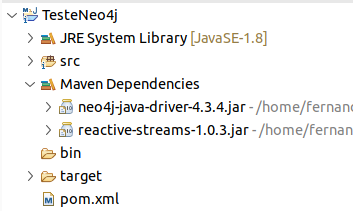
\includegraphics[width=0.5\textwidth]{imagens/dependenciasMaven}
	\caption{Dependências do Maven}
\end{figure}

Observamos que na pasta \textbf{Maven Dependencias} foi baixado a versão 2.8.1 do driver Jedis - Isso não é erro de digitação realmente o driver se escreve com "J".

\subsection{Exemplo Prático de uma Escola}
Estamos prontos para testarmos a conexão entre Redis e Java. Criamos um pequeno exemplo que nos auxiliará como teste, uma classe chamada \textbf{Escola} no pacote \textbf{decus.com} e inserimos nesta a seguinte codificação:
\begin{lstlisting}[]
package decus.com;

import java.text.SimpleDateFormat;
import java.util.Date;

import redis.clients.jedis.Jedis;

public class Escola {
	
	private String [] materias = new String[] {
	  "Matemática Computacional", "Programação", "Estatística",
  	  "SQL", "NoSQL", "Java", "Python", "Análise de Dados",
	  "Arquitetura de DW", "Big Data"
    };

	public static void main(String [] args) {
		new Escola().executar();
	}
	
	private void executar() {
		adicionarNotas();
	}
}
\end{lstlisting}

Nossa escola promove cursos mensais e temos um conjunto contendo todas as matérias que são aplicadas aos alunos. Ao término do curso é registrado o nome do aluno, a matéria e sua nota. Escolhemos o Redis para conter esses dados exatamente devido a sua característica de chave-valor.

No método principal que chama o executar, em Java não devemos programar no método "main". No executar colocamos uma chamada ao método criarAlunos() que terá a seguinte codificação:
\begin{lstlisting}[]
  private void adicionarNotas() {
	Jedis jedis = new Jedis();
	String data = new SimpleDateFormat("dd/MM/yyyy").format(new Date());
	String chave = "";
	String [] nomes = new String[] {
	  "Alice", "Miguel", "Sophia", "Arthur", "Helena", "Bernardo", "Valentina", 
	  "Heitor", "Laura", "Davi", "Isabella", "Lorenzo", "Manuela", "Théo", "Júlia", 
	  "Pedro", "Heloísa", "Gabriel", "Luiza", "Enzo", "Maria", "Luiza", "Matheus", 
	  "Lorena", "Lucas", "Lívia", "Benjamin", "Giovanna", "Nicolas", "Maria", 
	  "Eduarda", "Guilherme", "Beatriz", "Rafael", "Clara", "Joaquim", "Cecília"
	};
	String nome = "";
	for (int i = 0; i < 50; i++) {
	  nome = nomes[(int)(Math.random()*nomes.length)] + " " + nomes[(int)(Math.random()*nomes.length)];
  	  for (int j = 0; j < materias.length; j++) {
	    chave = "MAT" + i + "-" + j + "-" + data;
		jedis.hset(chave, "nome", nome);
		jedis.hset(chave, "materia", materias[j]);
		jedis.hset(chave, "nota", ""+(int)(Math.random()*11));
		jedis.close();
	  }
	}
	System.out.println("Notas Adicionadas");
  }
\end{lstlisting}

Obviamente como isto é um simples exemplo vamos adicionar as notas de uma forma totalmente aleatória.

Neste método temos a definição do objeto do Jedis que é responsável pela comunicação com o banco de dados que deve estar disponível na porta padrão. Criamos duas listas de nomes e matérias apenas para compor as notas que iremos inserir e ter dados mais elaborados. Teremos 50 alunos que ganharão nomes e sobrenomes completamente aleatórios com base na primeira lista, para cada um deles percorremos a lista de matéria e definimos uma chave que será composta por: "MAT" + valor de i (que é o número do aluno) + valor de j (que é o número da materia) e a data que estamos inserindo a informação. Assim temos a garantia que essa chave será única.

Para inserir a informação no objeto Jedis temos o método "hset" que recebe 3 parâmetros a chave, o nome do campo e o valor deste, e assim inserimos os campos nome, matéria e nota que será obtida também de forma aleatória (entre o valor de 0 a 10). Uma vez executado temos como resposta na console a mensagem "Notas Adicionadas" se verificamos no aplicativo "Another Redis Desktop Manager" teremos os seguintes dados:
\begin{figure}[H]
	\centering
	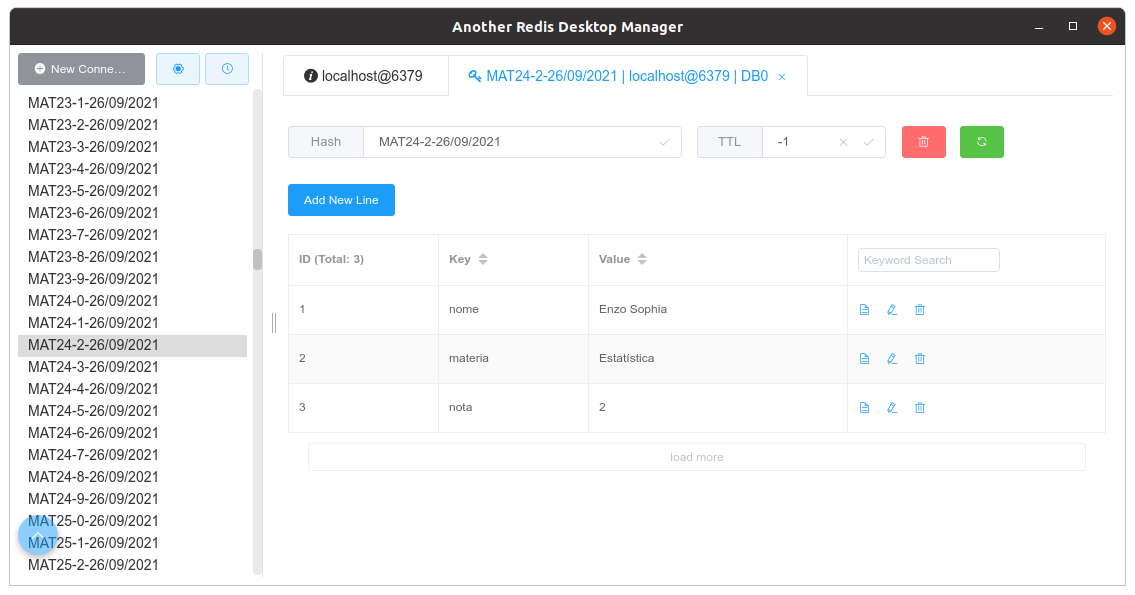
\includegraphics[width=0.8\textwidth]{imagens/notasAlunos}
	\caption{Another Redis Desktop Manager}
\end{figure}

Obviamente que os dados podem dar diferença pois o nome e as notas foram selecionados randomicamente.

\subsection{Localizações}
No método executar comentamos a chamada ao método "adicionarNotas()" e criamos outra para o método "trazerAluno(1)" que terá a seguinte codificação:
\begin{lstlisting}[]
  private void trazerAluno(int mat) {
	Jedis jedis = new Jedis();
	Set<String> nomes = jedis.keys("MAT" + mat + "-*");
	java.util.Iterator<String> it = nomes.iterator();
	String s;
	while (it.hasNext()) {
      s = it.next();
      System.out.print(jedis.hget(s, "nome") + " - ");
      System.out.print(jedis.hget(s, "materia") + " - ");
      System.out.println(jedis.hget(s, "nota"));
	}
	jedis.close();
  }	
\end{lstlisting}

As coisas no Redis são bem fáceis e rápidas, recebemos a matrícula e obtemos um conjunto (objeto Set) com todas as chaves que começam pela expressão "MAT1-" (como o valor que passamos foi 1) podemos utilizar esse método para realizar qualquer tipo de pesquisa, por exemplo "*-26/09/2021" trará todas as chaves do dia "26/09/2021". 

Percorremos esse conjunto e obtemos os dados que desejamos através do método "hget" no qual passamos a chave e o campo que desejamos. Ao executarmos teremos na console o nome do aluno, o nome da matéria e a nota obtida por esse.

Mas e se por exemplo desejamos saber a média geral das matérias dessa turma em cada matéria? Comentamos a chamada ao "trazerAluno(1)" no método executar por "mediaGeral()" e adicionamos a seguinte codificação:
\begin{lstlisting}[]
  private void mediaGeral() {
	Jedis jedis = new Jedis();
	String materia = "";
	for (int i = 0; i < materias.length; i++) { 
		int totNota = 0;
		int qtdNota = 0;
		Set<String> nomes = jedis.keys("*-"+i+"-*");
		java.util.Iterator<String> it = nomes.iterator();
		String s;
		while (it.hasNext()) {
			s = it.next();
			materia = jedis.hget(s, "materia");
			totNota += Integer.parseInt(jedis.hget(s, "nota"));
			qtdNota++;
		}
		System.out.println(materia + " - " + (totNota/qtdNota));
	}
	jedis.close();
  }	
\end{lstlisting}

E temos na saída da console cada uma das matérias e sua respectiva média.

\subsection{Eliminar Registro}
Assim como a consulta do registro é obtida através da chave o mesmo se aplica para a eliminação do mesmo, vamos comentar a chamada ao método "mediaGeral()" e chamar o método "eliminarAluno(1)" e adicionarmos a seguinte  codificação:
\begin{lstlisting}[]
  private void eliminarAluno(int mat) {
	Jedis jedis = new Jedis();
	Set<String> nomes = jedis.keys("MAT" + mat + "-*");
	java.util.Iterator<String> it = nomes.iterator();
	String s;
	while (it.hasNext()) {
		s = it.next();
		jedis.del(s);
	}
	jedis.close();
	System.out.println("Notas Eliminadas");
  } 	
\end{lstlisting}

Localizamos as chaves do aluno e executamos o método "del(chave)" para cada registro. Ou seja, extremamente simples e prático.

\subsection{Estrutura do objeto Jedis}
Aqui utilizamos o modelo estrutural de um Hash com mapeamento de um campo String como no de campo e seu respectivo valor e que pode ser aplicado para a grande maioria dos casos, porém existem outras estruturas no Redis que podem ser utilizadas com este conector.

\textbf{String}

É o modelo mais simples uma chave e um valor, pode ser utilizado por exemplo para uma associação de palavras como localidade e endereço:
\begin{lstlisting}[]
  jedis.set("Joaquim Lucas", "Qd 28 Casa 47 Rua Amélia Cidade Vale Alegre");
  jedis.set("Nicolas Cecília", "Qd 7 Casa 7 Rua Sete da Cidade Amarela");
  
  System.out.println(jedis.get("Joaquim Lucas"));
\end{lstlisting}

Ou seja, utilizamos o método "set(chave, valor)" para inserirmos a informação e o método "get(chave)" para obtê-la. Esse modelo também pode ser utilizado como uma camada de cache extremamente rápida e simples de se usar para solicitações HTTP recebidas de um aplicativo Web ou outros requisitos de cache. 

\textbf{Listas}

São listas de strings, classificadas por ordem de inserção e podem ser uma ferramenta ideal para implementar, por exemplo, filas de mensagens:
\begin{lstlisting}[]
jedis.lpush("tarefas", "Primeira tarefa do dia");
jedis.lpush("tarefas", "Segunda tarefa do dia");
jedis.lpush("tarefas", "Terceira tarefa do dia");
\end{lstlisting}

A cada comando "lpush(chave, valor)" uma nova tarefa é inserida. Para retirar usamos o comando:
\begin{lstlisting}[]
System.out.println(jedis.rpop("tarefas"));
\end{lstlisting}

Devemos lembrar que precisamos serializar qualquer objeto e persisti-lo como uma string, portanto, as mensagens na fila podem transportar dados mais complexos quando necessário.

\textbf{Conjuntos}

Trata de uma coleção não ordenada de Strings e que são bem úteis quando desejamos excluir membros repetidos, para adicionar elementos usamos:
\begin{lstlisting}[]
jedis.sadd("frutas", "abacate");
jedis.sadd("frutas", "manga");
jedis.sadd("frutas", "abacate");

Set<String> conjunto = jedis.smembers("frutas");
System.out.println(jedis.sismember("frutas", "abacate"));
\end{lstlisting}

As frutas do Java Set terão um tamanho de 2, a segunda adição de "abacate" foi ignorada. O método sismember permite que verifiquemos a existência de um membro específico rapidamente e mesmo com a resposta "true" se olharmos no nosso banco (usemos o aplicativo "Another Redis Desktop Manager") veremos que só existe uma única ocorrência para "abacate".
\begin{figure}[H]
	\centering
	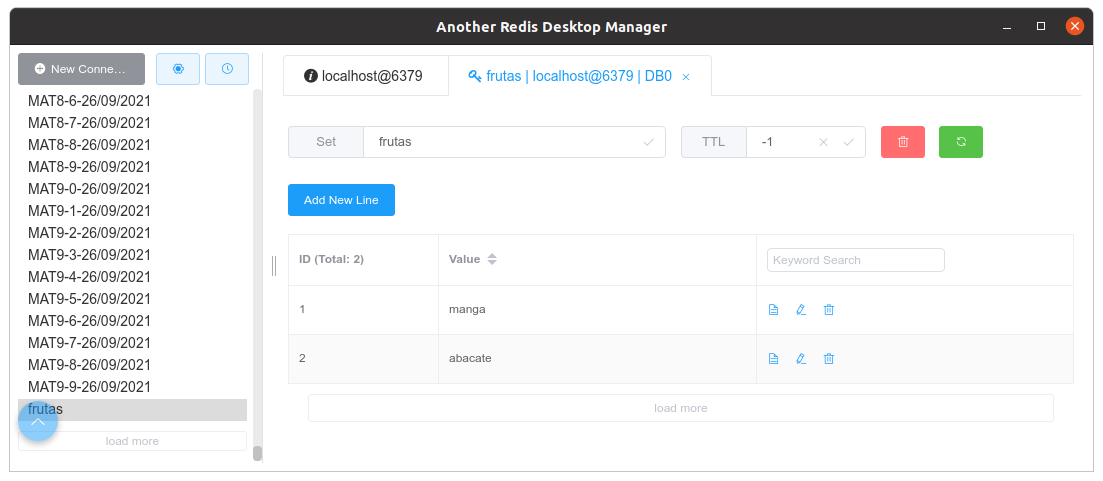
\includegraphics[width=0.8\textwidth]{imagens/frutas}
	\caption{Visão do Conjunto Frutas}
\end{figure}

\textbf{Conjuntos Ordenados}
São conjuntos classificados em que cada membro possui uma determinada classificação associada, que é usada para localizá-los. Podemos inserir alguns alunos e seus desempenhos da seguinte forma:
\begin{lstlisting}[]
Map<String, Double> desempenho = new HashMap<>();
desempenho.put("Aluno 1", 3000.0);
desempenho.put("Aluno 2", 1500.0);
desempenho.put("Aluno 3", 8200.0);
desempenho.put("Aluno 4", 2500.0);
desempenho.put("Aluno 5", 7500.0);
desempenho.put("Aluno 6", 6200.0);
desempenho.entrySet().forEach(playerScore -> {
  jedis.zadd("Desempenho", playerScore.getValue(), playerScore.getKey());
});	
\end{lstlisting}

E obtermos uma relação dos 3 melhores com a seguinte codificação:
\begin{lstlisting}[]
System.out.println("1o.: " + jedis.zrevrange("Desempenho", 0, 1).iterator().next());
System.out.println("2o.: " + jedis.zrevrange("Desempenho", 1, 2).iterator().next());
System.out.println("3o.: " + jedis.zrevrange("Desempenho", 2, 3).iterator().next());
\end{lstlisting}

Podemos utilizar de todas essas estruturas para criarmos uma aplicação extremamente veloz ou mesmo usar o Redis como um complementar para determinadas ações que precisamos aumentar os ganhos de velocidade.

\section{Python}
Python é uma linguagem de programação de alto nível, interpretada a partir de um script, Orientada a Objetos e de tipagem dinâmica. Foi lançada por Guido van Rossum em 1991. Não pretendo nesta apostila COMPARAR essa linguagem com Java (espero que nunca o faça), fica claro que os comandos são bem mais fáceis porém essas linguagens possuem diferentes propósitos.

Todos os comandos descritos abaixo foi utilizado no JupyterLab \cite{jupyteroficial}, então basta abrir um Notebook e digitá-los em cada célula conforme se apresentam.

\subsection{Proceder a Conexão}
Baixar o pacote necessário: \\
\codigo{ !pip install pymongo}

Importar os pacotes necessários: \\
\codigo{ from pymongo import MongoClient \\
	import random}

Neste caso estamos utilizando o pacote \textbf{random} somente para criarmos o mesmo exemplo já visto e escolher uma nota aleatória para casa aluno.

Nos conectamos ao servidor desta forma: \\
\codigo{ cliente = MongoClient('localhost', 27017)}
Ou: \\
\codigo{ cliente = MongoClient('mongodb://localhost:27017/')}

Listar as bases disponíveis: \\
\codigo{ cliente.list\_database\_names()) }

Nos conectamos a uma base desta forma: \\
\codigo{ db = cliente.escola}
Ou: \\
\codigo{ db = cliente['escola']}

Listar as coleções disponíveis: \\
\codigo{ cliente.list\_collection\_names()) }

Nos conectamos a uma coleção desta forma: \\
\codigo{ col = db.aluno}
Ou: \\
\codigo{ col = db['aluno']}

\subsection{Inserir documentos}
Inserir um único documento é uma questão de criar um dicionário e enviá-lo para a coleção: \\
\codigo{ mario = \{ "nome": "Mario da Silva", "nota": random.randint(1,11) \} \\
	col.insert\_one(mario) }

Inserir vários documentos é necessário criar uma lista de dicionários e enviar a lista para a coleção: \\
\codigo{ alunos = [ \\
	\phantom{x}\hspace{4pt} \{ "nome": "Aline Moraes", "nota": random.randint(1,11) \}, \\
	\phantom{x}\hspace{4pt} \{ "nome": "Soraya Gomes", "nota": random.randint(1,11) \} \\
	] \\
	col.insert\_many(alunos)
}

\subsection{Encontrar documentos}
Listar toda a coleção: \\
\codigo{ for doc in col.find(\{\}): \\
	\phantom{x}\hspace{4pt} print(doc)}

Listar toda a coleção de modo ordenado ascendente (ou descendente - valor -1): \\
\codigo{for doc in col.find(\{\}).sort("campo",1): \\
	\phantom{x}\hspace{4pt} print(doc)}

Quantos documentos existem na coleção: \\
\codigo{ col.count\_documents(\{\})}

Trazer o primeiro documento: \\
\codigo{ col.find\_one()}

Trazer um determinado documento: \\
\codigo{ col.find\_one(\{"nome": "Aline Moraes"\})}

Limitar a quantidade de documentos buscados (no caso 5): \\
\codigo{for doc in col.find(\{\}).limit(5): \\
	\phantom{x}\hspace{4pt} print(doc)}

Mostrar um determinado campo (e somente ele): \\
\codigo{for doc in col.find(\{\}): \\
	\phantom{x}\hspace{4pt} print(doc['col'])}

Trazer os documentos que possuem a nota maior que 5 e menor que 7: \\
\codigo{ for doc in col.find(\{"nota": \{"\$gt": 5, "\$lt": 7\}\}): \\
	\phantom{x}\hspace{4pt} print(doc)}

\subsection{Atualizar documentos}
* O lado da esquerda é o filtro de consulta e o lado do SET são os campos a alterar.

Alterar um documento que possui o nome "Mario da Silva": \\
\codigo{ col.update\_one(\{"nome": "Mario da Silva"\}, \{"\$set": \{"nota": 8\}\})}

Alterar os documentos que possuem a nota menor que 5: \\
\codigo{ col.update\_many(\{'nota': \{'\$lt': 5\}\}, \{'\$set': \{'nota': 4\}\})}

Eliminar um documento que possui o nome "Mario da Silva": \\
\codigo{ col.delete\_one(\{"nome": "Mario da Silva"\})}

Eliminar os documentos que possuem a nota menor que 5: \\
\codigo{ col.delete\_many(\{'nota': \{'\$lt': 5\}\})}

\subsection{Encerrar}
É boa prática fechar a base de dados: \\
\codigo{ cliente.close()}

Mas antes de encerramos realmente vejamos o seguinte programa completo em linguagem Python:

\begin{lstlisting}[]
from pymongo import MongoClient
from random import randint

# Passo 1: Conectar ao Mongo
cliente = MongoClient(port=27017)
db = cliente.negocio

# Passo 2: Criar Amostras de Dados
nomes = ['Kitchen', 'Espiritual', 'Mongo', 'Tastey', 'Big', 'Jr', 'Filho', 'City', 'Linux'
         'Tubarão', 'Gado', 'Sagrado', 'Solo', 'Sumo', 'Lazy', 'Fun', 'Prazer', 'Gula']
tipo_emp = ['LLC', 'Inc', 'Cia', 'Corp.']
tipo_coz = ['Pizza', 'Bar', 'Fast Food', 'Italiana', 'Mexicana',
            'Americana', 'Sushi', 'Vegetariana', 'Churrascaria']

for x in range(1, 501):
  nome1 = nomes[randint(0, (len(nomes)-1))]
  nome2 = nomes[randint(0, (len(nomes)-1))]
  tipoE = tipo_emp[randint(0, (len(tipo_emp)-1))]
  negocio = {
	'nome': nome1 + ' ' + nome2 + ' ' + tipoE,
	'nota': randint(1, 5),
	'cozinha': tipo_coz[randint(0, (len(tipo_coz)-1))]
  }  

# Passo 3: Inserir o objeto negócio no banco
result = db.restaurante.insert_one(negocio)

# Passo 4: Mostrar no console o Object ID do Documento
print('Criado {0} de 500 como {1}'.format(x, result.inserted_id))

# Passo 5: Mostrar mensagem final
print('500 Novos Negócios Culinários foram criados...')
cliente.close()
\end{lstlisting}

O programa está auto-documentado e criar uma base com 500 registros.

\section{Conclusão}
\textbf{Neo4j} é significativamente mais rápido na consulta de dados relacionados do que usar um banco de dados relacional tradicional. Além disso, uma única instância do Neo4j pode lidar com conjuntos de dados contendo três ordens de magnitude sem penalidades de desempenho. A independência do desempenho transversal no tamanho do gráfico é um dos principais aspectos que tornam o \textbf{Neo4j} torna-se um candidato ideal para resolver problemas de grafos, mesmo quando os conjuntos de dados são muito grandes.

Para auxiliar \textbf{Neo4j} a ser o mais rápido possível, dois sistemas de cache diferentes são usados: um cache de buffer e um de objetos. O primeiro tem como objetivo acelerar as consultas, ao armazenar uma cópia das informações recuperadas do gráfico, enquanto que o de objetos armazena versões otimizadas de nós, propriedades e relacionamentos para acelerar a travessia do grafo.

As principais linguagens de programação possuem suporte e aqui vimos apenas Java e Python, porém existem muitas outras como PHP, C, C++, C\#, JavaScript, Node.js, Ruby, R e Go. Esta apostila faz parte da série dos quatro tipos para Bancos de Dados no padrão NoSQL que estou tentando desmistificar e torná-los mais acessíveis tanto para as comunidades de Java e Python voltada especificamente para desenvolvedores ou cientistas de dados.
\begin{figure}[H]
	\centering
	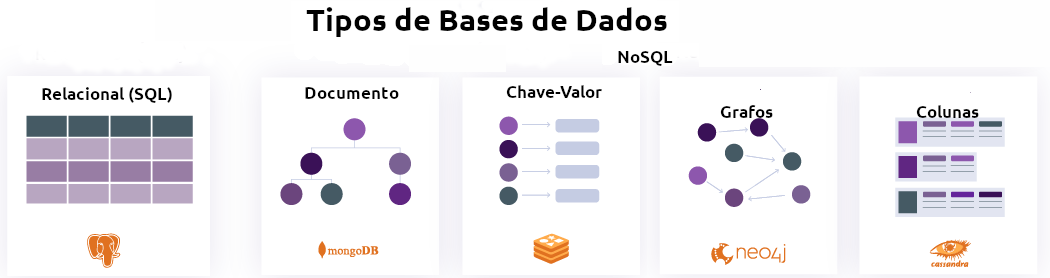
\includegraphics[width=0.8\textwidth]{../sty/NoSQL}
	\caption{Tipos de Bancos de Dados}
\end{figure}

Sou um entusiasta do mundo \textbf{Open Source} e novas tecnologias. Qual a diferença entre Livre e Open Source? \underline{Livre} significa que esta apostila é gratuita e pode ser compartilhada a vontade. \underline{Open Source} além de livre todos os arquivos que permitem a geração desta (chamados de arquivos fontes) devem ser disponibilizados para que qualquer pessoa possa modificar ao seu prazer, gerar novas, complementar ou fazer o que quiser. Os fontes da apostila (que foi produzida com o LaTex) está disponibilizado no GitHub \cite{github}. Veja ainda outros artigos que publico sobre tecnologia através do meu Blog Oficial \cite{fernandoanselmo}.

%-----------------------------------------------------------------------------
% REFERÊNCIAS
%-----------------------------------------------------------------------------
\begin{thebibliography}{8}
  \bibitem{neo4joficial} 
  Página do Neo4j \\
  \url{https://neo4j.com/}

  \bibitem{javaoficial} 
  Página do Oracle Java \\
  \url{http://www.oracle.com/technetwork/java}
  
  \bibitem{pythonoficial} 
  Página do Python \\
  \url{https://www.python.org}

  \bibitem{sts} 
  Editor Spring Tool Suite para códigos Java \\
  \url{https://spring.io/tools}

  \bibitem{jupyteroficial} 
  Página do Jupyter \\
  \url{https://jupyter.org/}

  	\bibitem{fernandoanselmo} 
	Fernando Anselmo - Blog Oficial de Tecnologia \\
	\url{http://www.fernandoanselmo.blogspot.com.br/}
	
	\bibitem{publicacao} 
	Encontre essa e outras publicações em \\
	\url{https://cetrex.academia.edu/FernandoAnselmo}
	
	\bibitem{github} 
	Repositório para os fontes da apostila \\
	\url{https://github.com/fernandoans/publicacoes}
\end{thebibliography}
  
\end{document}
